\documentclass{article}

% Workshop, double-blind review track at submission; accepted, now camera-ready
% (`final` added per NeurIPS 2026 formatting instructions).
\usepackage[dblblindworkshop, final]{neurips_2026}
\workshoptitle{AI for Drug Discovery -- Bridging the Translation Gap}

\usepackage[utf8]{inputenc}
\usepackage[T1]{fontenc}
\usepackage{hyperref}
\usepackage{url}
\usepackage{booktabs}
\usepackage{amsfonts}
\usepackage{amsmath}
\usepackage{nicefrac}
\usepackage{microtype}
\usepackage{xcolor}
\usepackage{longtable}
\usepackage{array}
\usepackage{tikz}
\usepackage{placeins}
\usepackage{float}
\usetikzlibrary{positioning}
\hypersetup{colorlinks=true, linkcolor=black, citecolor=black, urlcolor=black}

\title{From Model Scores to Discovery Decisions: Decision-Contract Evaluation of Tools for Molecular Generation and Docking}

\author{%
  Tuan Cao, Hai Luong, Tuan Dinh \\
  Life AI \\
  \texttt{tuan@lifeai.io, hai.luong@lifeai.io, tuan.dinh@lifeai.io}
}

\begin{document}

\maketitle

\begin{abstract}
Modern computational drug-discovery pipelines chain multiple stages, with competing tools at each. Yet tools are typically benchmarked in isolation using stage-specific metrics---such as molecular validity, uniqueness, property scores, or pose RMSD---that may not predict which tool best supports a downstream discovery decision. We introduce \textbf{DecisionBench-DD v1.0}, a decision-contract evaluation methodology that assesses tools within a frozen, auditable pipeline rather than a ready-made multi-target benchmark suite. We demonstrate it on two connected stages---molecular generation and docking---in a single ambroxol-conditioned glucocerebrosidase (GCase/\textit{GBA1}) case study comparing GenMol with MolMIM and GNINA with ligand-centered 15~\AA-cropped DiffDock-L. Although MolMIM led on uniqueness, diversity, QED, and synthetic accessibility, only 3/300 primary outputs passed the frozen chemical-qualification gates, versus 66/300 for GenMol. Post-hoc MolMIM reruns at \texttt{min\_similarity} 0.5 and 0.7 yielded 2/300 and 10/300 passers without reversing this ordering; neither rerun reached its requested threshold under independent ECFP4 recomputation. In redocking, the primary Top-1 endpoint did not reliably separate the dockers (3/14 versus 2/14), but GNINA recovered a near-native pose within five predictions for 8/14 versus 2/14, achieved lower best-of-five RMSD in all 14, and produced geometry-valid poses (70/70 versus 45/70). After downstream GNINA screening, 15/300 GenMol and 1/300 primary MolMIM outputs passed the structural proxy---a separation driven primarily by chemical qualification rather than demonstrated differential structural retention---while alternative rerankers changed redocking and screen counts in directions that cannot be signed without candidate-level ground truth. Tool rankings can therefore change when component metrics are replaced by task-specific constraints, frozen gates, and auditable advancement decisions.
\end{abstract}

\section{Introduction}

AI-enabled molecular-design tools are typically evaluated in isolation: generators by validity, uniqueness, diversity, or goal scores, and docking systems by pose RMSD or confidence [1--6]. An operational drug-discovery question is narrower and more consequential: \textbf{under a fixed budget and a specified molecular objective, which tool produces more candidates that survive the next decision?} Attractive component-level metrics can be misaligned with this task: high diversity aids exploration but can conflict with a seed-proximity constraint, and permissive proxy endpoints can silently acquire biological interpretations they were never validated to support.

We address this gap with \textbf{DecisionBench-DD v1.0}, organized around four principles: (1)~\textbf{freeze the decision contract}---gates and advancement rules are fixed before results are inspected; (2)~\textbf{compare like with like}---tools receive equivalent task information, with asymmetries made explicit; (3)~\textbf{measure decision yield}---performance propagates through the funnel using the requested count as denominator; and (4)~\textbf{audit transfer and proxy validity}---sensitivity analyses stay subordinate to the frozen primary analysis, and a proxy is not promoted to a biological claim without independent controls.

We instantiate this framework using ambroxol-conditioned analogue generation for GCase, encoded by \textit{GBA1}. Ambroxol is a marketed mucolytic reported to act as a pH-dependent mixed inhibitor and pharmacological chaperone of GCase [7,8], relevant to Gaucher disease and \textit{GBA1}-associated Parkinson's disease, and offering resolved structures, a known seed, and a mechanistically meaningful---but difficult---neutral-versus-acidic receptor-state question.

Our contributions are: an auditable generator-to-candidate funnel comparing GenMol [9] and MolMIM [10] under equal requested output counts; a task-specific GCase redocking validation comparing GNINA [4] with DiffDock-L [5,6]; a demonstrated ranking reversal between standard generator metrics and qualified yield, plus evidence that redocking-reranker gains do not by themselves establish improvement on an unlabeled candidate-screen proxy; and a frozen 16-candidate set with diversity, predictive ADMET, and exact-database-membership annotations, separated from experimental evidence.

\begin{figure}[t]
\centering
\resizebox{\linewidth}{!}{%
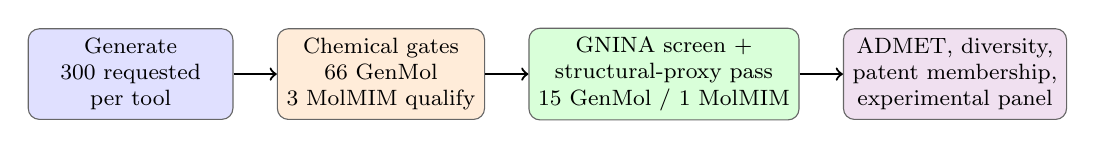
\begin{tikzpicture}[
  box/.style={draw=black!60, rounded corners, align=center, minimum height=1.15cm, minimum width=2.6cm, font=\footnotesize},
  arr/.style={->, thick},
  node distance=0.55cm
]
\node[box, fill=blue!12] (gen) {Generate\\300 requested\\per tool};
\node[box, fill=orange!15, right=of gen] (gate) {Chemical gates\\66 GenMol\\3 MolMIM qualify};
\node[box, fill=green!15, right=of gate] (dock) {GNINA screen +\\structural-proxy pass\\15 GenMol / 1 MolMIM};
\node[box, fill=violet!12, right=of dock] (down) {ADMET, diversity,\\patent membership,\\experimental panel};
\draw[arr] (gen) -- (gate);
\draw[arr] (gate) -- (dock);
\draw[arr] (dock) -- (down);
\end{tikzpicture}}
\caption{\textbf{DecisionBench-DD funnel.} Equal-output-budget generator outputs pass frozen chemical gates; qualified candidates enter GNINA candidate screening; primary structural passers enter downstream characterization. Every stage reports end-to-end yield against the original requested count, not just conditional retention (full attrition funnel in Appendix~B).}
\label{fig:funnel}
\end{figure}

\textbf{Related work.} MOSES [1] and GuacaMol [2] standardize generator metrics, but task-agnostic averages do not determine whether a generator respects a specific medicinal-chemistry contract. GenMol [9] and MolMIM [10] use discrete-diffusion and autoencoder-plus-CMA-ES generation respectively; GNINA [4] combines Vina-derived search with CNN scoring, while DiffDock/DiffDock-L [5,6] formulate blind docking as diffusion over pose degrees of freedom. PoseBusters showed low RMSD alone is insufficient since poses can be physically implausible [3]; we follow that lesson with a simplified proxy. DecisionBench-DD asks not only whether a tool performs well on its native benchmark but whether that ranking survives the gates and selectors used downstream.

\section{Methods}

The seed was ambroxol (\texttt{C1=C(C(=C(C=C1Br)Br)N)CNC2CCC(CC2)O}). Thresholds, gates, and scoring rules were version-controlled before each experiment, distinguishing mechanical corrections (no change to coordinates, connectivity, stereochemistry, ranks, or thresholds) from analytical amendments. Frozen analyses are primary; prespecified and post-hoc sensitivity analyses are labeled separately, and oracle best-of-$k$ results remain diagnostic. ``Chemical qualification'' means satisfying the declared cheminformatics gates; ``structural pass'' means satisfying a seed-relative \textbf{structural plausibility proxy}, not measured affinity, chaperone activity, cellular rescue, or developability.

\subsection{Experiment A: controlled generation}

GenMol and MolMIM each received the same seed and three independent requests of 100 molecules (300 per tool; an equal-output-budget, not equal-compute, comparison), via NVIDIA BioNeMo NIM (GenMol) and CMA-ES optimization with QED as target, \texttt{min\_similarity=0.3}, 100 particles, 10 iterations (MolMIM); full configurations are in Appendix A. Under our external ECFP4 evaluation (RDKit Morgan radius 2, 2048-bit, achiral), \texttt{min\_similarity=0.3} did not impose a hard 0.3 floor here; whether this reflects service-side similarity calculation, standardization, or soft enforcement could not be distinguished, so it is reported as a property of the tested configuration, not an intrinsic MolMIM limitation.

A molecule was chemically qualified only if RDKit-valid, unique within its replicate, not identical to ambroxol, with ECFP4 Tanimoto similarity to the seed in [0.30, 0.95), QED $\geq$0.50, SA score $\leq$5.0, molecular weight 200--550~Da, cLogP 0--5, TPSA $\leq$100~\AA$^{2}$, no PAINS alerts, and no \textbf{new} Brenk alert: since ambroxol itself triggers a Brenk aniline alert, an atom-mapped substructure check confirmed whether a candidate's alert was the seed's own instance (non-disqualifying) or an additional occurrence (disqualifying; Appendix B).

We reported validity, within-replicate uniqueness, pooled internal diversity (one minus mean pairwise ECFP4 Tanimoto), median seed similarity, QED, synthetic accessibility, alert pass rates, and the primary qualified yield $Y_{\mathrm{chemical}} = N_{\mathrm{pass\ all\ gates}} / N_{\mathrm{requested}}$.

\subsection{Experiment B: GCase redocking}

Fourteen experimentally resolved GCase--ligand complexes were frozen before docking (11 allosteric-site, three active-site-chaperone); receptor/ligand protonation and exact GNINA flags are in Appendix~C. DiffDock-L exposes no native pocket-restriction parameter, so for comparability its receptor input was cropped to a 15~\AA\ radius around the same box center; we refer to it throughout as \textbf{DiffDock-L with ligand-centered 15~\AA\ receptor cropping}, not unrestricted blind DiffDock-L.

We calculated heavy-atom, symmetry-aware \textbf{in-place} RMSD using RDKit \texttt{CalcRMS} (no realignment): Success@1 (top-ranked poses at RMSD $\leq$2~\AA) primary, with Success@5, median Top-1/best-of-five RMSD, and a geometry-validity proxy as secondary endpoints. Fifteen DiffDock-L poses carried a reproducible representation artifact, corrected before scoring with no coordinate/rank change (targeted fix, not an independent replicate; full audit in Appendix~D). Two fixed selectors---CNN\_VS descending and minimized affinity ascending---were applied as bounded sensitivity analyses (\S4.1: CNN\_VS depends on CNNaffinity) without replacing the native CNNscore Top-1 analysis.

\subsection{Candidate screening and downstream characterization}

All 69 chemically qualified candidates (66 GenMol, 3 MolMIM) plus four controls were docked with GNINA against two matched structures of \textit{GBA1} c.1226A$>$G, p.Asn409Ser (legacy N370S): PDB 3KEH (pH 7.4) and 3KE0 (acidic pH) [11], using an active-site box from superposing the validation-set 3GXF chain (146 five-pose jobs). A primary structural pass on 3KEH required five returned poses, a geometry-valid Top-1 pose, a ligand heavy atom within 4.5~\AA\ of a side-chain carboxylate oxygen of \emph{either} catalytic Glu235 or Glu340, and Top-1 CNNaffinity $\geq$ ambroxol's; neutral-minus-acidic differences were exploratory, not a gate.

Primary passers were characterized by ECFP4/Murcko scaffold diversity, physicochemical properties, and ADMET-AI predictions [12], and screened for exact-structure membership against a SureChEMBL snapshot and ZINC in-stock using MolBloom [13]---an approximate check, not similarity, novelty, patentability, or freedom-to-operate analysis.

Generator yields carry bootstrap 95\% confidence intervals (2{,}000 resamples of the pooled 300 outcomes, treated as independent Bernoulli draws, which does not model between-replicate correlation); final pipeline yields use exact binomial 95\% intervals under the same assumption. Because the redocking set held only 14 complexes, paired outcomes and effect direction were emphasized over null-hypothesis claims, and the exact sign test on discordant Success@5 outcomes was treated as exploratory since it was not specified in the frozen analysis plan.

\section{Results}

\subsection{Standard generator metrics and qualified yield disagree}

\begin{table}[t]
  \caption{Equal-output-budget generator scorecard (300 requested molecules per tool).}
  \label{tab:generator}
  \centering
  \footnotesize
  \begin{tabular}{lrr}
    \toprule
    Metric & GenMol & MolMIM \\
    \midrule
    Validity & \textbf{100.0\%} & 99.0\% \\
    Within-replicate uniqueness & 67.0\% & \textbf{100.0\%} \\
    Internal diversity & 0.668 & \textbf{0.842} \\
    Median Tanimoto to seed & \textbf{0.361} & 0.167 \\
    Mean QED & 0.543 & \textbf{0.742} \\
    Mean SA score (lower is better) & 3.77 & \textbf{3.10} \\
    PAINS pass rate & \textbf{99.7\%} & 99.3\% \\
    \textbf{Qualified yield, 95\% CI} & \textbf{22.0\% (17.3--26.7\%)} & \textbf{1.0\% (0.0--2.3\%)} \\
    \bottomrule
  \end{tabular}
\end{table}

MolMIM was stronger on uniqueness, diversity, QED, and had lower (better) SA scores; GenMol had higher validity and PAINS pass rate and stayed closer to the seed (Table 1). The downstream decision reversed this ranking: 66/300 GenMol molecules passed all chemical gates versus 3/300 MolMIM. Scored independently rather than cumulatively (Appendix~B), the similarity gate alone passes only 4.0\% of MolMIM's valid outputs versus 76.7\% of GenMol's, while QED alone shows the opposite pattern (97.0\% vs.\ 61.7\%). Across \texttt{min\_similarity} settings of 0.3, 0.5, and 0.7, entry into the similarity band was non-monotonic (12/300, 4/300, 14/300); median similarity stayed 0.167 and the maximum across all settings was 0.468, with neither rerun meeting its requested threshold. The tested hosted MolMIM service did not reliably enforce this constraint under our independent ECFP4 definition; the comparison characterizes the deployed configuration and leaves untested whether an effectively enforced, definition-matched constraint could satisfy the contract. Conditional on entering the similarity band, 66/148 GenMol and 3/12 primary MolMIM candidates survived the remaining gates (44.6\% vs.\ 25.0\%)---too small a MolMIM denominator to establish a downstream generator difference. The second-largest marginal separation, at the seed-relative Brenk gate, is also reference-conditioned: MolMIM's greater scaffold drift reduced mapping to Ambroxol's allowlisted aniline, so the reversal reflects the contract's seed-proximity requirement propagating, not generally poorer chemistry. GenMol's uniqueness was lower, but attrition was distributed across the funnel (67.0\% unique $\to$ 49.3\%~similarity-qualified $\to$ 29.0\%~QED-qualified $\to$ 22.0\%~all-gates-qualified). Raw Brenk incidence was also misleading: every GenMol output carried at least one alert, but most reflected the seed-inherent aromatic amine rather than a new liability, and the position-aware rule avoided rejecting the seed scaffold while still catching additional instances.

\subsection{Redocking separates sampling, ranking, and validity}

\begin{table}[t]
  \caption{Frozen GCase redocking results.}
  \label{tab:redocking}
  \centering
  \footnotesize
  \begin{tabular}{lrr}
    \toprule
    Metric & GNINA & DiffDock-L, cropped \\
    \midrule
    Success@1 (RMSD $\leq$2~\AA) $\uparrow$ & \textbf{21.4\% (3/14)} & 14.3\% (2/14) \\
    Success@5 (RMSD $\leq$2~\AA) $\uparrow$ & \textbf{57.1\% (8/14)} & 14.3\% (2/14) \\
    Median Top-1 RMSD $\downarrow$ & 4.64~\AA & \textbf{4.26~\AA} \\
    Median best-of-five RMSD $\downarrow$ & \textbf{1.55~\AA} & 4.01~\AA \\
    Lower best-of-five RMSD $\uparrow$ & \textbf{14/14} & 0/14 \\
    Top-1 geometry-valid $\uparrow$ & \textbf{100\%} & 78.6\% \\
    All poses geometry-valid $\uparrow$ & \textbf{100\% (70/70)} & 64.3\% (45/70) \\
    \bottomrule
  \end{tabular}
\end{table}

The primary Success@1 comparison was inconclusive (two GNINA-only, one DiffDock-L-only, one shared success; Table 2), and median Top-1 RMSD also favored cropped DiffDock-L numerically. Secondary evidence favored GNINA: it recovered a near-native pose within five outputs for 8/14 complexes versus 2/14 (exploratory exact sign test $p=0.031$), with lower best-of-five RMSD in every complex and geometry-proxy validity for all 70 poses. Of those 8, 5 were not ranked first (ranking failure) and the remaining 6/14 complexes had no near-native pose in Top-5 (unrecovered); both remain limitations. Fixed CNN\_VS and minimized-affinity selectors raised Success@1 to 4/14 and 5/14 (versus 3/14 native; \S4.1 on transfer). The validation set is allosteric-heavy (11/14); on the 3 active-site complexes (the candidate screen's advancement-gate type, \S2.3), GNINA's Success@1/5 was 0/3 and 2/3 vs.\ 1/3 and 1/3 for DiffDock-L (Appendix~D) --- too few to resolve independently.

\subsection{End-to-end yield preserves the generator reversal}

All 146 candidate/control jobs completed and returned five poses; 16 candidates (15 GenMol, 1 MolMIM) passed the frozen Top-1 structural proxy, giving a final end-to-end yield of 5.00\% (95\% exact CI 2.83--8.11\%) for GenMol versus 0.33\% (0.01--1.84\%) for MolMIM (Appendix~B); this gap is driven principally by chemical qualification, not docking, since the conditional retention estimates (15/66 vs.\ 1/3, i.e.\ 22.7\% vs.\ 33.3\%) cannot establish a generator difference with so small a MolMIM denominator. An any-pose Top-5 oracle identified 11 additional GenMol candidates (0 MolMIM), yielding 27/69 possible passes. CNN\_VS yielded 21 total passes and minimized affinity 12, versus 16 native; neither change is interpretable as better/worse qualification without candidate-level ground truth, and CNN\_VS is mechanically non-independent of the CNNaffinity-thresholded gate (\S4.1). The 16 Top-1 candidates remained primary; the 11 rescues were kept only as an exploratory reserve.

The 16 primary passers occupied eight ECFP4 clusters and ten Murcko scaffolds (QED 0.53--0.78, SA 2.97--4.76, 15/16 with no Lipinski violation). Predictive ADMET exposed trade-offs absent from the docking proxy: nine candidates had higher predicted hERG-inhibition than ambroxol, while GM\_053 and GM\_057 had lower predicted hERG liability with reduced predicted BBB permeability (used for prioritization, not as gates). No exact-structure membership was detected for any primary passer in the tested 30.9-million-compound SureChEMBL snapshot; one gave a positive ZINC in-stock membership indication (Bloom filters admit false positives, not false negatives, so this requires confirmation, not a confirmed match).

\subsection{Paired receptor-state scores do not establish pH-dependent pharmacology}

Ambroxol's neutral-minus-acidic CNNaffinity difference was positive but small ($+0.057$), passing the one frozen, version-controlled directional sanity check. The three other docked molecules (isofagomine, P9V, P8Y) were not frozen as directional controls and instead favored the acidic receptor; only 23/57 interpretable candidate comparisons favored the neutral state. These are reported descriptively, not as a failed control check: the endpoint was never calibrated against measured pH-dependent binding, and crystallization pH, receptor-protonation, and ligand-protonation are distinct choices that two structures at different pH do not, alone, validate as a pH-dependent-binding simulation. We retain the scores as exploratory ranking information only, not evidence of pH-dependent binding, lysosomal release, or chaperoning.

\section{Discussion}

\subsection{The relevant comparison depends on the decision}

This case study has no universal winner. MolMIM's more unique, diverse set with better average QED/SA suits broad exploration; in the frozen primary comparison, GenMol's narrower analogue-generation focus delivered a far higher qualified-molecule rate (22.0\% vs.\ 1.0\%) and final structural-passer rate (5.00\% vs.\ 0.33\%) per requested molecule, an ordering the post-hoc \texttt{0.7} sensitivity setting narrowed but did not reverse---the right choice depends on whether the goal is ``explore broadly'' or ``produce usable analogues under this contract.'' The docking comparison shows the same dependence: cropped DiffDock-L had a slightly lower median Top-1 RMSD, while GNINA had better Top-5 recovery, best-of-five RMSD, and validity, so a one-pose workflow is unresolved while a five-pose workflow favors GNINA.

GNINA's correct-pose recovery rose from 3/14 at Top-1 to 8/14 within five poses (5 ranking failures, 6 unrecovered; \S3.2). CNN\_VS and minimized affinity raised redocking Success@1 to 4/14 and 5/14, and changed candidate-screen passes to 21 and 12 (from 16 native; Appendix~E)---not a transfer failure, since the endpoints differ and neither change is signable as improvement without candidate-level ground truth. Rerankers need independent, task-matched validation before replacing Top-$k$ retention with the best retrospective rule.

The paired 3KEH/3KE0 screen (\S3.4) illustrates the same lesson: it passed only its own frozen Ambroxol sanity check, not a validated control battery, so such deltas generate hypotheses, not substitutes for neutral-pH binding, catalytic-modulation, or cellular-rescue assays. DecisionBench-DD v1.0 has too few complexes (14, including 11 allosteric) or, in the frozen primary screen, only three MolMIM candidates, for superiority claims, and a cropped DiffDock-L. GenMol's per-replicate qualified counts (30/100, 29/100, 7/100) show more spread than the pooled 22.0\% estimate's CI reflects (unreplayable exactly; Appendix~A). The allosteric/active-site mismatch (\S3.2) limits the active-site-only gate; CNNaffinity/ADMET-AI/SureChEMBL are not experimental evidence. \textbf{In conclusion, tool rankings can reverse once frozen constraints propagate through a funnel:} the 16 candidates are a prioritization output, not validated chaperones, and selectors need independent, task-matched validation.

\section*{References}

\small

[1] Polykovskiy, D. et al. Molecular Sets (MOSES): A Benchmarking Platform for Molecular Generation Models. \textit{Frontiers in Pharmacology} 11, 565644 (2020). \url{https://doi.org/10.3389/fphar.2020.565644}

[2] Brown, N., Fiscato, M., Segler, M. H. S. \& Vaucher, A. C. GuacaMol: Benchmarking Models for De Novo Molecular Design. \textit{Journal of Chemical Information and Modeling} 59, 1096--1108 (2019). \url{https://doi.org/10.1021/acs.jcim.8b00839}

[3] Buttenschoen, M., Morris, G. M. \& Deane, C. M. PoseBusters: AI-based docking methods fail to generate physically valid poses or generalise to novel sequences. \textit{Chemical Science} 15, 3130--3139 (2024). \url{https://doi.org/10.1039/D3SC04185A}

[4] McNutt, A. T. et al. GNINA 1.0: molecular docking with deep learning. \textit{Journal of Cheminformatics} 13, 43 (2021). \url{https://doi.org/10.1186/s13321-021-00522-2}

[5] Corso, G., St\"ark, H., Jing, B., Barzilay, R. \& Jaakkola, T. DiffDock: Diffusion Steps, Twists, and Turns for Molecular Docking. \textit{International Conference on Learning Representations} (2023). \url{https://openreview.net/forum?id=kKF8_K-mBbS}

[6] Corso, G. et al. Deep Confident Steps to New Pockets: Strategies for Docking Generalization. \textit{International Conference on Learning Representations} (2024). \url{https://openreview.net/forum?id=UfBIxpTK10}

[7] Maegawa, G. H. B. et al. Identification and Characterization of Ambroxol as an Enzyme Enhancement Agent for Gaucher Disease. \textit{Journal of Biological Chemistry} 284, 23502--23516 (2009). \url{https://doi.org/10.1074/jbc.M109.012393}

[8] Bendikov-Bar, I., Maor, G., Filocamo, M. \& Horowitz, M. Ambroxol as a pharmacological chaperone for mutant glucocerebrosidase. \textit{Blood Cells, Molecules, and Diseases} 50, 141--145 (2013). \url{https://doi.org/10.1016/j.bcmd.2012.10.007}

[9] Lee, S. et al. GenMol: A Drug Discovery Generalist with Discrete Diffusion. arXiv:2501.06158 (2025). \url{https://arxiv.org/abs/2501.06158}

[10] Reidenbach, D., Livne, M., Ilango, R. K., Gill, M. \& Israeli, J. Improving Small Molecule Generation using Mutual Information Machine. arXiv:2208.09016 (2022). \url{https://arxiv.org/abs/2208.09016}

[11] Wei, R. R. et al. X-ray and Biochemical Analysis of N370S Mutant Human Acid $\beta$-Glucosidase. \textit{Journal of Biological Chemistry} 286, 299--308 (2011). \url{https://doi.org/10.1074/jbc.M110.150060}

[12] Swanson, K. et al. ADMET-AI: a machine learning ADMET platform for evaluation of large-scale chemical libraries. \textit{Bioinformatics} 40, btae416 (2024). \url{https://doi.org/10.1093/bioinformatics/btae416}

[13] Medina, J. \& White, A. D. Bloom filters for molecules. \textit{Journal of Cheminformatics} 15, 95 (2023). \url{https://doi.org/10.1186/s13321-023-00765-1}

\clearpage
\appendix

These appendices are supplementary material and are not counted against the five-page main-text limit. All raw manifests, per-run logs, candidate structures, hashes, and code referenced below are version-controlled in the project repository; the tables here are condensed, verified extracts. Repository: \url{https://github.com/lifeai-io/DecisionBench-DD}.

\FloatBarrier
\section{Generator configurations and replicate-level metrics}
\label{app:a}

\textbf{Frozen invocation parameters.} Both tools received the identical seed SMILES \texttt{C1=C(C(=C(C=C1Br)Br)N)CNC2CCC(CC2)O} and were called three times as independent replicates (100 molecules requested per call); neither API exposes a documented random-seed field.

\begin{table}[h]
\centering
\footnotesize
\begin{tabular}{ll}
\toprule
GenMol NIM parameter & Value \\
\midrule
num\_molecules & 100 (per replicate) \\
temperature & 1.0 (documented default) \\
noise & 1.0 (documented default) \\
gamma & 0.0 \\
min\_add\_len & 24 \\
scoring & QED \\
unique / filter & false / false (post-hoc filtering done by our own gates, not the API) \\
\bottomrule
\end{tabular}
\hspace{1em}
\begin{tabular}{ll}
\toprule
MolMIM NIM parameter & Value \\
\midrule
num\_molecules & 100 (per replicate) \\
algorithm & CMA-ES \\
property\_name & QED \\
minimize & false \\
min\_similarity & 0.3 (requested; \S2.1 notes this was not observed as a hard floor) \\
particles & 100 \\
iterations & 10 \\
\bottomrule
\end{tabular}
\end{table}

\textbf{Per-replicate breakdown} (100 requested per replicate; source: \texttt{chemical\_gate\_audit.csv}):

\begin{table}[h]
\centering
\footnotesize
\begin{tabular}{lrrr}
\toprule
GenMol & Replicate 1 & Replicate 2 & Replicate 3 \\
\midrule
Valid & 100 & 100 & 100 \\
Within-replicate unique & 84 & 49 & 68 \\
Chemically qualified & 30 & 29 & 7 \\
\bottomrule
\end{tabular}
\hspace{1em}
\begin{tabular}{lrrr}
\toprule
MolMIM & Replicate 1 & Replicate 2 & Replicate 3 \\
\midrule
Valid & 97 & 100 & 100 \\
Within-replicate unique & 97 & 100 & 100 \\
Chemically qualified & 1 & 1 & 1 \\
\bottomrule
\end{tabular}
\end{table}

GenMol's 100.0\% validity has run-to-run stdev 0.0\,pp; MolMIM's 99.0\% pooled validity has stdev 1.7\,pp (driven entirely by replicate 1). Qualified counts sum to 66 (GenMol) and 3 (MolMIM), matching Table~1.

\textbf{Summed vs.\ pooled uniqueness.} GenMol's within-replicate unique counts sum to $84+49+68=201$, matching the ``67.0\% unique'' figure reported in Table~1. This is \emph{not} the same as the number of distinct molecules across all three replicates pooled together: recomputing uniqueness over the union of all three GenMol replicates gives \textbf{200} distinct canonical structures, i.e.\ exactly one molecule recurred across two different replicates. To be precise about what each number drives: $Y_{\mathrm{chemical}} = N_{\mathrm{pass\ all\ gates}}/N_{\mathrm{requested}}$ always has a fixed denominator of 300 requested molecules; within-replicate deduplication is one of the cumulative gates that determines which outputs can reach the numerator, not a component of the denominator. The pooled count (200) is reported here only as a diagnostic and was not used in any gate or headline statistic.

\textbf{MolMIM \texttt{min\_similarity} sensitivity (post-hoc, reviewer-requested).} Run after inspecting the primary results, using the identical seed, pipeline, and frozen gates but overriding only \texttt{min\_similarity} (\texttt{decisionbench\_dd\_eval/run\_generation\_sensitivity.py}; source manifests in \texttt{runs\_sensitivity/}, scored results in \texttt{results\_sensitivity/}):

\begin{table}[h]
\centering
\footnotesize
\begin{tabular}{lrrrrr}
\toprule
\texttt{min\_similarity} & Rep.\ 1 & Rep.\ 2 & Rep.\ 3 & Pooled qualified & Yield (95\% CI) \\
\midrule
0.3 (primary) & 1 & 1 & 1 & 3/300 & 1.0\% (0.0--2.3\%) \\
0.5 & 1 & 1 & 0 & 2/300 & 0.7\% (0.0--1.7\%) \\
0.7 & 4 & 1 & 5 & 10/300 & 3.3\% (1.3--5.3\%) \\
\bottomrule
\end{tabular}
\caption{MolMIM chemically-qualified counts (of 100 requested per replicate) as \texttt{min\_similarity} varies. Median externally-recomputed ECFP4 Tanimoto-to-seed was 0.167 at all three settings, consistent with the primary-run finding that this parameter does not impose a hard similarity floor under our independent RDKit recomputation. GenMol's pooled qualified yield (22.0\%, unaffected by this rerun) remains far above MolMIM's at every tested setting.}
\end{table}

\textbf{Sensitivity scorecard (distributional detail).} Table~3 reports only pass/fail counts; the observed generated-molecule distributions differed across the requested settings, most visibly in the upper tail:

\begin{table}[h]
\centering
\footnotesize
\begin{tabular}{lrr}
\toprule
Metric & \texttt{0.5} & \texttt{0.7} \\
\midrule
Valid & 295/300 & 297/300 \\
Unique among valid & 100.0\% & 99.7\% \\
Mean ECFP4 similarity & 0.170 & 0.178 \\
Median ECFP4 similarity & 0.167 & 0.167 \\
Frozen similarity-band pass & 4/300 & 14/300 \\
Maximum similarity & 0.458 & 0.468 \\
Mean QED & 0.755 & 0.783 \\
Mean SA & 3.34 & 3.17 \\
Internal diversity & 0.839 & 0.837 \\
Chemical pass & 2/300 & 10/300 \\
Structural pass & 0/300 & 2/300 \\
\bottomrule
\end{tabular}
\caption{Sensitivity-run distributional detail. Source: molecule-level sensitivity outputs in the project repository. Median externally recomputed ECFP4 similarity was 0.167 at both settings. The observed \texttt{0.7} sample had higher mean and maximum similarity than the \texttt{0.5} sample, but without controlled seeds this descriptive difference cannot be attributed to \texttt{min\_similarity}. No output reached external ECFP4 similarity 0.5 or 0.7 (maximum observed 0.468).}
\end{table}

\FloatBarrier

\textbf{End-to-end GNINA re-screen of the sensitivity candidates.} The 2 (\texttt{min\_similarity=0.5}) and 10 (\texttt{0.7}) qualified candidates above were carried through the identical candidate-screen pipeline (\S2.3: same digest-pinned GNINA image, boxes, gate; \texttt{decisionbench\_dd\_docking/prepare\_candidate\_screen\_ligands.py} / \texttt{run\_candidate\_screen\_gnina.py} / \texttt{score\_candidate\_screen.py}, run on a separate GPU machine from the primary screen):

\begin{table}[h]
\centering
\footnotesize
\begin{tabular}{lrr}
\toprule
\texttt{min\_similarity} & Structural-proxy pass & End-to-end yield (95\% CI) \\
\midrule
0.3 (primary) & 1/300 & 0.33\% (0.01--1.84\%) \\
0.5 & 0/300 & 0.00\% (0.00--1.22\%) \\
0.7 & 2/300 & 0.67\% (0.08--2.39\%) \\
\midrule
GenMol (fixed, unaffected) & 15/300 & 5.00\% (2.83--8.11\%) \\
\bottomrule
\end{tabular}
\caption{End-to-end structural-proxy yield of the MolMIM sensitivity candidates. Source: candidate-screen sensitivity outputs in the project repository, against GenMol's frozen primary yield (unaffected by this rerun, since only MolMIM was regenerated). The two \texttt{0.7} structural passers are post-hoc sensitivity outputs only and were not added to the frozen 16-candidate primary set characterized in \S3.3 and Appendices E--G. GenMol's frozen 15/300 yield remained higher than MolMIM's 0/300 and 2/300 sensitivity yields at every tested \texttt{min\_similarity} setting. The re-scored Ambroxol threshold differed from the primary value by 0.0009, consistent with hardware-dependent floating-point variation, although its source was not experimentally isolated. This difference was smaller than every candidate's pass/fail margin and changed no classification.}
\end{table}

\FloatBarrier
\section{Chemical-gate definitions and attrition audit}
\label{app:b}

\textbf{Gate order and thresholds} (frozen protocol v1.2, \texttt{qualification\_gates\_v1.0.json}): valid (RDKit parses) $\to$ unique (first occurrence within its own replicate) $\to$ not an exact Ambroxol copy $\to$ ECFP4 Tanimoto to seed in $[0.30,0.95)$ (radius 2, 2048-bit) $\to$ QED $\geq 0.50$ $\to$ SA (Ertl) $\leq 5.0$ $\to$ MW $200$--$550$~Da $\to$ cLogP $0$--$5$ $\to$ TPSA $\leq 100$~\AA$^2$ $\to$ zero PAINS\_A/B/C hits (absolute gate) $\to$ no new, unmapped Brenk alert instance.

\textbf{Seed-relative Brenk rule.} Ambroxol itself triggers an aniline Brenk alert, so a candidate's Brenk occurrence is disqualifying only if it does \emph{not} correspond, atom-for-atom, to the seed's own alert instance. Correspondence is computed via \texttt{rdFMCS.FindMCS} (atom compare: elements; bond compare: order; ring-matches-ring-only) between seed and candidate, and a candidate occurrence is seed-inherited only if every atom of some seed instance maps under this correspondence to exactly the candidate's matched atom set. This instance-level rule (v1.2) replaced an earlier, alert-\emph{type}-only rule (v1.1) that could not distinguish the seed's own aniline from an unrelated second aniline introduced elsewhere; both amendments were made from the seed molecule alone, before any GenMol/MolMIM comparison data existed.

\begin{table}[h]
\centering
\footnotesize
\begin{tabular}{lrrrr}
\toprule
Stage (cumulative) & \multicolumn{2}{c}{GenMol} & \multicolumn{2}{c}{MolMIM} \\
 & count & \% of 300 & count & \% of 300 \\
\midrule
Requested & 300 & 100.0\% & 300 & 100.0\% \\
Valid & 300 & 100.0\% & 297 & 99.0\% \\
Unique (within replicate) & 201 & 67.0\% & 297 & 99.0\% \\
Not exact seed & 199 & 66.3\% & 297 & 99.0\% \\
Similarity band [0.30, 0.95) & 148 & 49.3\% & 12 & 4.0\% \\
QED $\geq$0.50 & 87 & 29.0\% & 11 & 3.7\% \\
SA $\leq$5.0 & 84 & 28.0\% & 11 & 3.7\% \\
MW 200--550~Da & 83 & 27.7\% & 11 & 3.7\% \\
cLogP 0--5 & 70 & 23.3\% & 9 & 3.0\% \\
TPSA $\leq$100~\AA$^2$ & 68 & 22.7\% & 8 & 2.7\% \\
No PAINS & 68 & 22.7\% & 8 & 2.7\% \\
\textbf{Chemically qualified} & \textbf{66} & \textbf{22.0\%} & \textbf{3} & \textbf{1.0\%} \\
\bottomrule
\end{tabular}
\caption{Full attrition funnel underlying Table~1 (pooled across the three replicates per tool). Source: \texttt{chemical\_gate\_audit.csv} / \texttt{results/summary.md}.}
\label{tab:attrition-funnel}
\end{table}

Brenk instance rates (of valid molecules): GenMol -- any alert 100.0\%, all-seed-inherited 84.3\%, $\geq$1 new/unmapped instance (used for qualification) 15.7\%. MolMIM -- any alert 51.2\%, all-seed-inherited 0.3\%, $\geq$1 new instance 50.8\%.

\textbf{Marginal (independent) per-gate pass rates.} The cumulative funnel above conflates gate stringency with gate position: a gate applied late only screens molecules that already survived every earlier gate. Each gate is in fact evaluated independently per molecule (\texttt{decisionbench\_dd\_eval/gates.py:evaluate\_gates}, not short-circuited), so the marginal pass rate of every gate against the full valid population is recoverable directly from \texttt{results/molecule\_level.csv} without rerunning anything:

\begin{table}[h]
\centering
\footnotesize
\begin{tabular}{lrr}
\toprule
Gate (applied independently) & GenMol (\% of 300 valid) & MolMIM (\% of 297 valid) \\
\midrule
Within-replicate unique & 67.0\% & 100.0\% \\
Not exact seed & 99.3\% & 100.0\% \\
Similarity $\geq$0.30 & \textbf{76.7\%} & \textbf{4.0\%} \\
Similarity $<$0.95 & 99.3\% & 100.0\% \\
QED $\geq$0.50 & \textbf{61.7\%} & \textbf{97.0\%} \\
SA $\leq$5.0 & 97.7\% & 100.0\% \\
MW 200--550~Da & 98.7\% & 100.0\% \\
cLogP 0--5 & 69.0\% & 97.0\% \\
TPSA $\leq$100~\AA$^2$ & 97.7\% & 97.3\% \\
No PAINS & 99.7\% & 99.3\% \\
No new Brenk instance & 84.3\% & 49.2\% \\
\midrule
\textbf{Cumulative final qualified} & \textbf{22.0\%} & \textbf{1.0\%} \\
\bottomrule
\end{tabular}
\caption{Marginal per-gate pass rate (each gate scored alone against all valid outputs, not against survivors of earlier gates), versus the cumulative funnel in Table~\ref{tab:attrition-funnel}. The similarity gate alone rejects 96\% of MolMIM's valid outputs (4.0\% marginal pass) while rejecting only 23\% of GenMol's (76.7\%); QED alone shows the opposite pattern (97.0\% vs.\ 61.7\%). The largest marginal separation occurs at the similarity gate, although the seed-relative Brenk gate also contributes (84.3\% vs.\ 49.2\%).}
\end{table}

\textbf{End-to-end candidate yield.} Continuing the funnel above through docking (\S2.3) to the frozen structural-pass gate (\S3.3):

\begin{table}[h]
\centering
\footnotesize
\begin{tabular}{lrr}
\toprule
Stage & GenMol & MolMIM \\
\midrule
Requested & 300 & 300 \\
Chemically qualified & 66 (22.0\%) & 3 (1.0\%) \\
Primary structural pass & 15 & 1 \\
Conditional structural retention & 22.7\% & 33.3\% \\
\textbf{Final yield, 95\% exact CI} & \textbf{5.00\% (2.83--8.11\%)} & \textbf{0.33\% (0.01--1.84\%)} \\
\bottomrule
\end{tabular}
\caption{End-to-end candidate yield (conditional retention shown separately; MolMIM denominator is only three). Summarized in the main text, \S3.3.}
\end{table}

\FloatBarrier
\section{14-complex structural-validation set and preparation provenance}
\label{app:c}

\begin{table}[h]
\centering
\footnotesize
\begin{tabular}{lccccc}
\toprule
PDB ID & Site & Res.\ (\AA) & Ligand & RSCC & Occ.\ \\
\midrule
9F9Z & allosteric & 2.28 & A1IBI & 0.893 & 0.80 \\
9FA3 & allosteric & 1.36 & A1IBC & 0.896 & 0.62 \\
9FA6 & allosteric & 1.49 & A1IBG & 0.935 & 0.76 \\
9FAD & allosteric & 1.80 & A1IBD & 0.942 & 0.72 \\
9FAL & allosteric & 1.39 & A1IBQ & 0.972 & 0.84 \\
9FAY & allosteric & 1.40 & A1IBR & 0.967 & 0.93 \\
9FAZ & allosteric & 1.63 & A1IBP & 0.893 & 0.71 \\
9FB2 & allosteric & 1.14 & A1IBO & 0.969 & 0.93 \\
9FDI & allosteric & 1.41 & A1IB1 & 0.931 & 0.85 \\
8P3E & allosteric & 1.75 & WSI & 0.918 & 1.00 \\
8P41 & allosteric & 1.83 & WYC & 0.894 & 1.00 \\
3GXF & active-site-chaperone & 2.40 & IFM & 0.994 & 1.00 \\
6Q1N & active-site-chaperone & 2.53 & P9V & 0.842 & 1.00 \\
6Q1P & active-site-chaperone & 2.80 & P8Y & 0.922 & 1.00 \\
\bottomrule
\end{tabular}
\caption{Frozen 14-complex redocking set (RSCC/occupancy from RCSB electron-density/occupancy metadata, used for ligand-instance selection). Ligand instance chosen per case from the deposited alternate/occupancy records, not by RMSD or docking outcome.}
\end{table}

\textbf{Receptor preparation.} PDB2PQR 3.7.1, AMBER force field, PROPKA titration, pH 7.4 (single frozen physiological pH applied uniformly, not per-structure). \textbf{Ligand preparation.} dimorphite-dl 2.0.2, pH 7.4, with a frozen, content-based (not positional) microstate tie-break rule. \textbf{Docking box.} GNINA: crystal-ligand heavy-atom extent $+6$~\AA\ per side, supplied via \texttt{-{}-center\_x/y/z -{}-size\_x/y/z}. DiffDock-L: no native pocket-restriction flag exists, so its receptor input was cropped to a 15~\AA\ radius around the same box center (69--122 of 497--1988 residues retained depending on structure) -- an approximation of pocket-conditioning, explicitly not equivalent to GNINA's box search, and not native/uncropped DiffDock-L.

\FloatBarrier
\section{Pose-level redocking results and representation-artifact audit}
\label{app:d}

\textbf{Commands.} GNINA (dockerized \texttt{gnina/gnina:latest}, GPU): \texttt{gnina -r <receptor> -l <ligand> -{}-center\_x/y/z -{}-size\_x/y/z -{}-num\_modes 5 -{}-exhaustiveness 8 -{}-seed 42 -{}-cnn\_scoring rescore}. The \texttt{:latest} tag is not itself immutable, but the run manifest recorded the resolved content digest actually pulled at execution time: \texttt{gnina/gnina@sha256:9da3dc61eef272cecb60798933a9a977d028c47024845fdf1f05a941ce5e25a2} (the same digest was independently resolved for the later candidate-screen run, \S2.3). DiffDock-L (dockerized \texttt{rbgcsail/diffdock}, commit \texttt{85c49b6} of the gcorso/DiffDock repository, batch/CSV inference mode, documented defaults \texttt{inference\_steps=20}, \texttt{samples\_per\_complex=5}): \texttt{micromamba run -n diffdock python -m inference -{}-config default\_inference\_args.yaml -{}-protein\_ligand\_csv <csv> -{}-out\_dir <dir> -{}-samples\_per\_complex 5}, run inside \texttt{docker run -{}-rm -{}-gpus all rbgcsail/diffdock}. The hosted DiffDock NIM API was explicitly \emph{not} used, since its underlying checkpoint version is not independently confirmed to be DiffDock-L.

\begin{table}[h]
\centering
\footnotesize
\begin{tabular}{lc rrcc rrcc}
\toprule
 & & \multicolumn{4}{c}{GNINA} & \multicolumn{4}{c}{DiffDock-L, cropped} \\
PDB & Site & Top-1 & Best-5 & S@1 & S@5 & Top-1 & Best-5 & S@1 & S@5 \\
\midrule
9F9Z & allo & 0.89 & 0.89 & Y & Y & 2.99 & 2.66 & N & N \\
9FA3 & allo & 2.21 & 2.21 & N & N & 3.70 & 3.70 & N & N \\
9FA6 & allo & 5.89 & 1.26 & N & Y & 7.12 & 6.36 & N & N \\
9FAD & allo & 6.04 & 1.03 & N & Y & 5.67 & 4.32 & N & N \\
9FAL & allo & 5.24 & 4.76 & N & N & 9.43 & 5.97 & N & N \\
9FAY & allo & 5.56 & 5.56 & N & N & 9.74 & 5.59 & N & N(5) \\
9FAZ & allo & 0.88 & 0.87 & Y & Y & 7.28 & 6.13 & N & N(5) \\
9FB2 & allo & 7.27 & 0.82 & N & Y & 3.03 & 2.82 & N & N(5) \\
9FDI & allo & 1.53 & 1.18 & Y & Y & 1.39 & 1.39 & Y & Y \\
8P3E & allo & 4.17 & 4.17 & N & N & 4.81 & 4.72 & N & N \\
8P41 & allo & 5.11 & 5.11 & N & N & 6.23 & 5.62 & N & N \\
3GXF & active & 3.43 & 1.62 & N & Y & 1.73 & 1.73 & Y & Y \\
6Q1N & active & 8.73 & 1.49 & N & Y & 2.73 & 2.51 & N & N \\
6Q1P & active & 3.40 & 2.62 & N & N & 2.91 & 2.91 & N & N \\
\bottomrule
\end{tabular}
\caption{Per-complex RMSD (\AA) and success at RMSD $\leq$2~\AA. Parenthesized counts under DiffDock-L S@5 indicate poses affected by the sulfonamide-charge artifact (see below); ``allo''/``active'' abbreviate allosteric/active-site-chaperone.}
\end{table}

Site-stratified aggregates: GNINA allosteric ($n$=11) Success@1/5 = 27.3\%/54.5\%; GNINA active-site ($n$=3) = 0.0\%/66.7\%. DiffDock-L allosteric = 9.1\%/9.1\%; DiffDock-L active-site = 33.3\%/33.3\%. The validation set is allosteric-heavy (11/14) while the candidate screen's advancement gate is active-site-only (\S4.1), a mismatch noted as a limitation in the main text.

\textbf{Representation-artifact audit.} Three complexes (9FAY, 9FAZ, 9FB2), five poses each (15 total), had a DiffDock-L output-representation artifact: a neutral tertiary sulfonamide nitrogen assigned a spurious $+1$ formal charge. Neutralizing this charge (\texttt{rmsd.\_fix\_known\_pose\_charge\_artifact}) was necessary to restore atom correspondence for RMSD scoring; a direct programmatic comparison confirmed zero change to atomic coordinates, connectivity, stereochemical tags, or pose ranking before vs.\ after the fix. This was a targeted representation correction, not an independent stochastic replicate: under the pinned container and invocation, repeated executions produced byte-identical poses for all 14 cases, and the interface exposed no seed control, so stochastic uncertainty could not be estimated. Geometry-validity failures are independent of this artifact and reflect the frozen geometry-validity proxy (valid valence; bonded distances within 0.7--2.2~\AA; no nonbonded heavy-atom pair below 1.5~\AA): DiffDock-L's Top-1 pose is invalid for exactly 3/14 complexes (9FAL, 9FAY, 9FB2; 11/14 = 78.6\% valid, matching Table~2), while 11/14 complexes have at least one invalid pose somewhere in their five-pose set (only 9F9Z, 9FAD, and 6Q1N have all five poses geometry-valid).

\FloatBarrier
\section{Candidate-level selector turnover (69 candidates)}
\label{app:e}

Per-candidate Top-1 pass (\textbf{P}) or fail (\textbf{--}) under each of the three frozen, non-fitted selectors (native CNNscore rank-1, CNN\_VS descending, minimized-affinity ascending), against the fixed structural-pass bar defined in \S2.3. Column totals: native 16/69, CNN\_VS 21/69, minimized-affinity 12/69 (matches \S3.3). Full per-pose CNNscore/CNNaffinity/CNN\_VS/minimizedAffinity values underlying this table are archived in \texttt{candidate\_selector\_turnover.csv}.

\textbf{Pass-set overlap.} CNN\_VS retains all 16 native passers and adds 5 new ones (union 21; Jaccard $16/21=0.762$). Minimized affinity retains 8 of the 16 native passers, loses 8, and adds 4 new ones (union 20; Jaccard $8/20=0.400$), the larger of the two turnovers. Overlap alone does not indicate which selector is more accurate; it only quantifies how much the ranked set changes.

\begin{longtable}{lcccc}
\toprule
Candidate & Tool & Native & CNN\_VS & Min.\ affinity \\
\midrule
\endfirsthead
\toprule
Candidate & Tool & Native & CNN\_VS & Min.\ affinity \\
\midrule
\endhead
GM\_001 & genmol & -- & -- & -- \\
GM\_002 & genmol & -- & -- & -- \\
GM\_003 & genmol & -- & -- & -- \\
GM\_004 & genmol & -- & -- & -- \\
GM\_005 & genmol & -- & -- & -- \\
GM\_006 & genmol & -- & -- & -- \\
GM\_007 & genmol & P & P & -- \\
GM\_008 & genmol & -- & -- & -- \\
GM\_009 & genmol & -- & P & -- \\
GM\_010 & genmol & -- & -- & -- \\
GM\_011 & genmol & -- & -- & -- \\
GM\_012 & genmol & -- & -- & -- \\
GM\_013 & genmol & -- & -- & -- \\
GM\_014 & genmol & -- & -- & -- \\
GM\_015 & genmol & P & P & P \\
GM\_016 & genmol & -- & -- & -- \\
GM\_017 & genmol & -- & -- & P \\
GM\_018 & genmol & -- & -- & -- \\
GM\_019 & genmol & -- & -- & -- \\
GM\_020 & genmol & -- & -- & -- \\
GM\_021 & genmol & -- & -- & -- \\
GM\_022 & genmol & -- & -- & -- \\
GM\_023 & genmol & -- & -- & -- \\
GM\_024 & genmol & P & P & P \\
GM\_025 & genmol & -- & -- & -- \\
GM\_026 & genmol & -- & -- & P \\
GM\_027 & genmol & -- & -- & -- \\
GM\_028 & genmol & -- & -- & -- \\
GM\_029 & genmol & -- & -- & -- \\
GM\_030 & genmol & -- & -- & -- \\
GM\_031 & genmol & P & P & -- \\
GM\_032 & genmol & P & P & -- \\
GM\_033 & genmol & P & P & -- \\
GM\_034 & genmol & P & P & -- \\
GM\_035 & genmol & P & P & -- \\
GM\_036 & genmol & -- & P & -- \\
GM\_037 & genmol & -- & -- & -- \\
GM\_038 & genmol & -- & -- & -- \\
GM\_039 & genmol & P & P & P \\
GM\_040 & genmol & -- & -- & -- \\
GM\_041 & genmol & -- & P & P \\
GM\_042 & genmol & -- & -- & -- \\
GM\_043 & genmol & -- & -- & P \\
GM\_044 & genmol & -- & -- & -- \\
GM\_045 & genmol & -- & -- & -- \\
GM\_046 & genmol & -- & P & -- \\
GM\_047 & genmol & P & P & P \\
GM\_048 & genmol & -- & -- & -- \\
GM\_049 & genmol & -- & -- & -- \\
GM\_050 & genmol & -- & -- & -- \\
GM\_051 & genmol & -- & -- & -- \\
GM\_052 & genmol & -- & -- & -- \\
GM\_053 & genmol & P & P & P \\
GM\_054 & genmol & P & P & P \\
GM\_055 & genmol & P & P & -- \\
GM\_056 & genmol & -- & -- & -- \\
GM\_057 & genmol & P & P & -- \\
GM\_058 & genmol & -- & -- & -- \\
GM\_059 & genmol & -- & -- & -- \\
GM\_060 & genmol & -- & -- & -- \\
GM\_061 & genmol & -- & -- & -- \\
GM\_062 & genmol & -- & -- & -- \\
GM\_063 & genmol & -- & -- & -- \\
GM\_064 & genmol & P & P & P \\
GM\_065 & genmol & -- & -- & -- \\
GM\_066 & genmol & -- & P & -- \\
MM\_001 & molmim & -- & -- & -- \\
MM\_002 & molmim & P & P & P \\
MM\_003 & molmim & -- & -- & -- \\
\bottomrule
\end{longtable}

\FloatBarrier
\section{ADMET-AI provenance and raw outputs}
\label{app:f}

\textbf{Provenance.} \texttt{admet\_ai} package v2.0.1 (v2-line; PAINS/BRENK/NIH\_alert columns confirm v2, not v1); \texttt{chemprop} v2.3.1; bundled model-directory SHA-256 \texttt{c59e05b0...ee32bb9} (full hash in \texttt{admet\_predictions.md}); repository git commit \texttt{b277d3c}; exact command \texttt{python -m decisionbench\_dd\_docking.predict\_admet}. All values below are Chemprop-RDKit model predictions trained on Therapeutics Data Commons benchmarks, not experimental measurements; the full $\sim$50-endpoint output (including DrugBank-approved-drug percentile ranks) is in \texttt{admet\_predictions.csv}.

\begin{longtable}{lrrrrrrrr}
\toprule
Candidate & hERG & AMES & DILI & ClinTox & BBB & HIA & CYP3A4 & t$_{1/2}$ (h) \\
\midrule
\endfirsthead
\toprule
Candidate & hERG & AMES & DILI & ClinTox & BBB & HIA & CYP3A4 & t$_{1/2}$ (h) \\
\midrule
\endhead
CTRL\_AMBROXOL & 0.798 & 0.168 & 0.142 & 0.222 & 0.922 & 0.999 & 0.075 & 52.3 \\
GM\_007 & 0.885 & 0.118 & 0.152 & 0.270 & 0.940 & 0.999 & 0.077 & 76.4 \\
GM\_015 & 0.759 & 0.040 & 0.587 & 0.139 & 0.729 & 1.000 & 0.534 & 58.8 \\
GM\_024 & 0.851 & 0.160 & 0.213 & 0.355 & 0.920 & 0.999 & 0.171 & 48.1 \\
GM\_031 & 0.840 & 0.703 & 0.335 & 0.319 & 0.961 & 1.000 & 0.317 & 53.0 \\
GM\_032 & 0.781 & 0.749 & 0.573 & 0.260 & 0.949 & 1.000 & 0.450 & 53.2 \\
GM\_033 & 0.852 & 0.396 & 0.400 & 0.241 & 0.909 & 1.000 & 0.413 & 59.7 \\
GM\_034 & 0.857 & 0.189 & 0.198 & 0.188 & 0.899 & 0.999 & 0.225 & 54.4 \\
GM\_035 & 0.766 & 0.256 & 0.269 & 0.182 & 0.825 & 0.999 & 0.213 & 54.8 \\
GM\_039 & 0.919 & 0.131 & 0.247 & 0.185 & 0.894 & 1.000 & 0.475 & 55.0 \\
GM\_047 & 0.776 & 0.654 & 0.442 & 0.288 & 0.941 & 1.000 & 0.599 & 41.9 \\
GM\_053 & 0.315 & 0.127 & 0.281 & 0.235 & 0.551 & 0.808 & 0.031 & 15.3 \\
GM\_054 & 0.919 & 0.402 & 0.066 & 0.103 & 0.789 & 0.968 & 0.132 & 48.8 \\
GM\_055 & 0.987 & 0.389 & 0.427 & 0.312 & 0.933 & 1.000 & 0.905 & 58.7 \\
GM\_057 & 0.352 & 0.126 & 0.181 & 0.221 & 0.540 & 0.784 & 0.026 & 15.7 \\
GM\_064 & 0.918 & 0.129 & 0.371 & 0.269 & 0.853 & 1.000 & 0.629 & 59.5 \\
MM\_002 & 0.783 & 0.366 & 0.269 & 0.192 & 0.918 & 0.998 & 0.504 & 44.1 \\
\bottomrule
\end{longtable}

Risk endpoints (hERG/AMES/DILI/ClinTox/CYP3A4) are predicted probabilities where \emph{lower} is safer; BBB/HIA are predicted probabilities where \emph{higher} is favorable; half-life is predicted directly in hours (not log-hours). \textbf{Invalid (negative) clearance predictions}: 2/17 hepatocyte, 6/17 microsome, flagged via \texttt{Clearance\_*\_valid} columns in the CSV rather than silently reported -- a negative value is a regression-model extrapolation artifact, not evidence of unusually good stability. \textbf{On BRENK\_alert}: 15/16 candidates trigger it, but this is the same single seed-inherited dibrominated-aniline instance already qualified against the frozen v1.2 seed-relative gate (Appendix~B), not 15 independently discovered liabilities -- ADMET-AI's raw check has no knowledge of that upstream allowlisting.

\FloatBarrier
\section{Exact-membership scope and experimental-validation panel}
\label{app:g}

\textbf{Membership-check scope.} molbloom's SureChEMBL Bloom filter (FPR $0.000025$; filter file SHA-256 \texttt{fba90fba...50e99786}, a downloaded external artifact, not re-derivable from source) tests only exact-structure membership; it is not a similarity, Markush-claim, tautomer/salt, or freedom-to-operate search, and admits false positives but not false negatives. Ambroxol was sanity-checked and correctly returns \texttt{True}.

\begin{longtable}{lcc}
\toprule
Candidate & In SureChEMBL & In ZINC in-stock \\
\midrule
\endfirsthead
\toprule
Candidate & In SureChEMBL & In ZINC in-stock \\
\midrule
\endhead
CTRL\_AMBROXOL & True & True \\
GM\_007 & False & False \\
GM\_015 & False & False \\
GM\_024 & False & False \\
GM\_031 & False & True \\
GM\_032 & False & False \\
GM\_033 & False & False \\
GM\_034 & False & False \\
GM\_035 & False & False \\
GM\_039 & False & False \\
GM\_047 & False & False \\
GM\_053 & False & False \\
GM\_054 & False & False \\
GM\_055 & False & False \\
GM\_057 & False & False \\
GM\_064 & False & False \\
MM\_002 & False & False \\
\bottomrule
\end{longtable}

No exact-structure membership was detected in the tested SureChEMBL snapshot for any of the 16 primary candidates; GM\_031 separately gives a positive ZINC in-stock indication, useful for rapid procurement but requiring its own compound-identity and prior-art check, not an availability claim.

\textbf{Frozen experimental-validation panel (v1.1.1, pre-data).} The 16 primary passers are split into a Tranche~1 panel of 6 and a Tranche~2 reserve of 10, both frozen before any wet-lab data exists:

\begin{table}[H]
\centering
\footnotesize
\begin{tabular}{ll}
\toprule
Candidate & Role \\
\midrule
GM\_035 & Comparatively balanced predicted profile \\
GM\_015 & Binding/efficacy anchor \\
MM\_002 & Orthogonal-generator representative \\
GM\_034 & Ambroxol-like anchor \\
GM\_054 & Prediction-challenge comparator \\
GM\_057 & Low-toxicity / pH-sensitivity lead \\
\bottomrule
\end{tabular}
\end{table}

Tranche~2 reserve (10): GM\_007, GM\_024, GM\_031, GM\_032, GM\_033, GM\_039, GM\_047, GM\_053, GM\_055, GM\_064.

\textbf{Assay sequence (Tier 1--3).} Tier 1: analytical solubility and cytotoxicity, GCase binding/stabilization plus a sign-agnostic catalytic-modulation assay across pH (reporting inhibition IC$_{50}$ and/or activation EC$_{50}$ plus a pH-selectivity ratio, since Ambroxol is a pH-dependent mixed inhibitor, not an activator). Tier 2: cellular chaperone-rescue assay, hERG counterscreen (thallium-flux triage; the 30$\times$ hERG-to-cellular-efficacy index requires a validated patch-clamp IC$_{50}$, not the triage signal), and metabolic (microsomal/hepatocyte) stability. Tier 3: oral (Caco-2) and CNS permeability, with passive CNS permeability (PAMPA-BBB) explicitly reported separately from a required MDCK-MDR1/BCRP-competent transporter-efflux assay. The Tier1$\to$Tier2 cytotoxicity gate branches for stabilization-only vs.\ catalytic-modulator candidates; hepatocyte-stability is an optimization flag, not a mandatory ALL-pass criterion. Full assay definitions, frozen statistical analysis plan (effect sizes, CIs, multiple-comparison correction), and SOP annex requirements are in \texttt{experimental\_validation\_panel\_v1.0.md}.

\textbf{Amendment history.} v1.0 (frozen 2026-08-26) required neutral-pH GCase ``activation,'' which self-contradicted this same document's description of Ambroxol as a pH-dependent inhibitor; v1.1 (same day) replaced this with a sign-agnostic binding/stabilization plus catalytic-modulation design. v1.1.1 (2026-08-26T23:31:21Z UTC, external review) corrected: mixed-type (not competitive) inhibitor language; N370S/N409S recognized as the same variant (\textit{GBA1} c.1226A\textgreater{}G, p.Asn409Ser) under legacy vs.\ HGVS numbering; an underspecified frozen statistical analysis plan; a branch-undefined cytotoxicity gate; a self-contradictory hepatocyte-stability gate; PAMPA-BBB/transporter-efflux conflation; and hERG/cellular-assay execution rigor. Compound membership (Tranche 1/2) was unchanged throughout all amendments.

\end{document}
